%\linenumbers
\chapter{Introducción}

El \emph{aprendizaje máquina}\footnote{Traducido como \emph{machine learning} en inglés, tiene como objetivo desarrollar técnicas que les permitan a las computadoras aprender.} es un área dentro de la \emph{ciencia de datos}\footnote{Traducido como \emph{data science} en inglés, involucra métodos para extraer conocimiento de datos, eso con la finalidad de que haya un mejor entendimiento de los datos.} que puede ayudar a crear dichos modelos para tener una más eficiente visualización cuando se trabaja con una gran cantidad de datos, que es lo que se requiere para el presente trabajo. El área de la ciencia de datos es muy útil ya que permite trabajar con grandes cantidades de datos aminorando la cantidad de tiempo empleado en la creación de gráficos que permitan visualizar los datos. El crear modelos para la visualización de datos ayuda a observar con mayor claridad los datos para encontrar relaciones entre ellos.


La tarea en el presente proyecto es utilizar modelos para visualizar las relaciones entre los contaminantes del aire y salud pública. Para la realización de los experimentos se tienen datos de ingresos hospitalarios provenientes de la base de datos de la Secretaría de Salud del Gobierno de México \cite{f1}. También se tienen registros de los niveles de algunos contaminantes del aire presentes en el área metropolitana de Monterrey, capturados por las estaciones de monitoreo pertenecientes al Sistema Integral de Monitoreo Ambiental (SIMA) \cite{f2} mostradas en la figura \ref{estaciones} y en el cuadro \ref{tab:Coordenadas estaciones}.

\begin{figure}[h!]
\setcounter{figure}{0} % por culpa de sciposter
\captionsetup{type=figure} % por culpa de sciposter
\begin{center}
   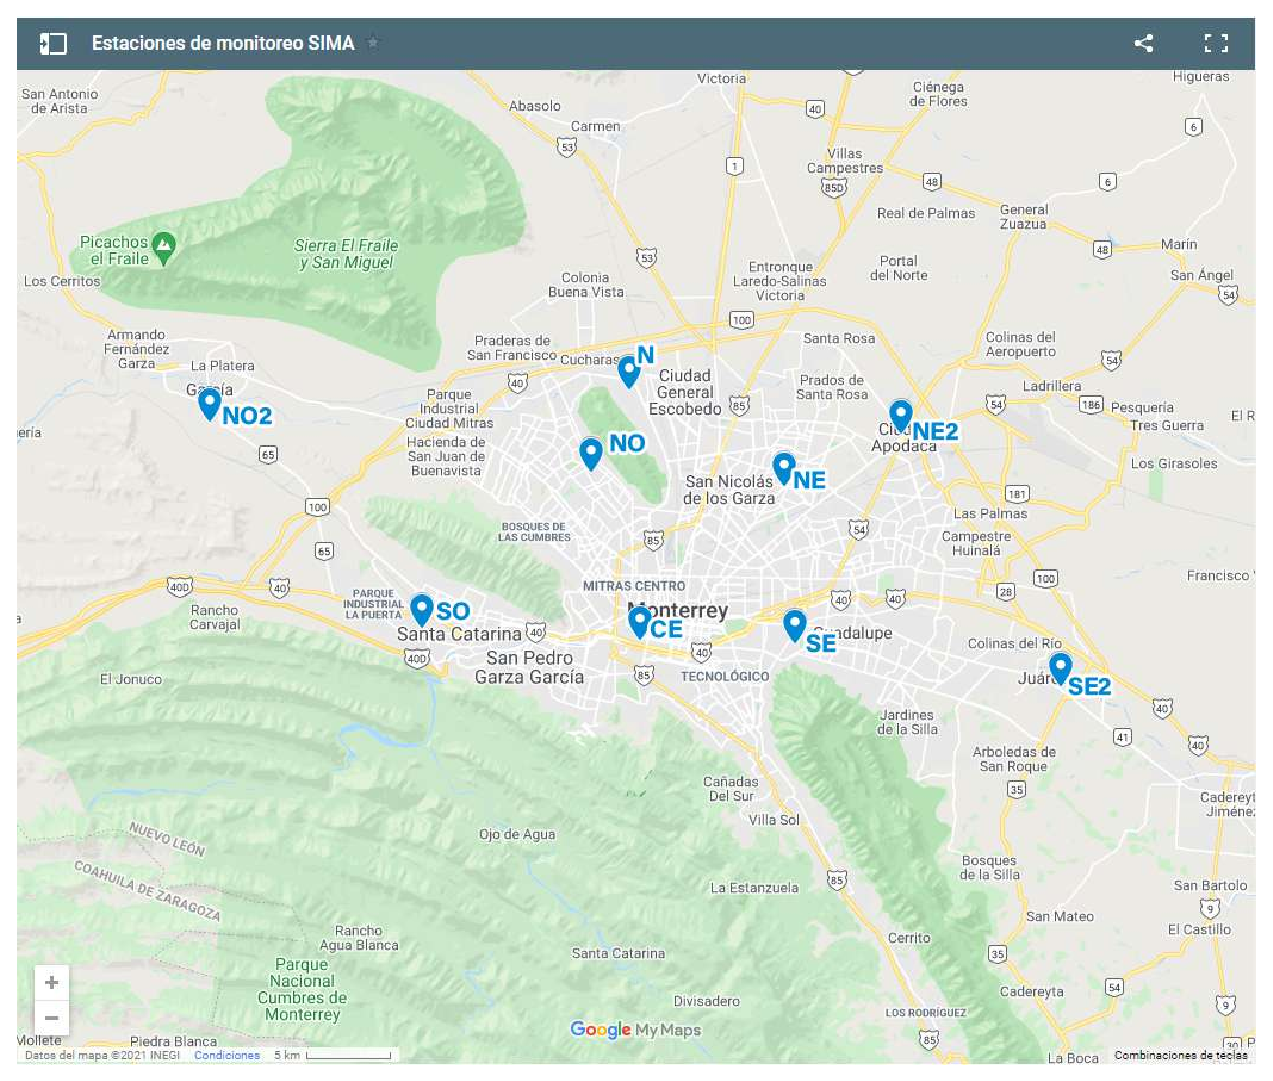
\includegraphics[trim=50 50 50 50,clip,width=1\textwidth]{mapa_estaciones.eps}
   \end{center}
    \caption{Localización de las estaciones de monitoreo de la calidad del aire.}
    \label{estaciones}
\end{figure}

%Las herramientas utilizadas en la presente investigación se muestran en el cuadro \ref{tab:Coordenadas estaciones}.
\begin{table}[H]
	{\centering
		\caption{Coordenadas de las estaciones de monitoreo de la calidad del aire.}
		\begin{tabular}{|c|c|c|}
			\hline 
			Estación & Latitud & Longitud\\
			\hline
			SE & 25.668 & -100.249\\
			\hline
			NE & 25.750 & -100.255\\
			\hline
			CE & 25.670 & -100.338\\
			\hline
			NO & 25.757 & -100.366\\
			\hline
			SO & 25.676 & -100.464\\
			\hline
			NO2 & 25.783 & -100.586\\
			\hline
			NE2 & 25.777 & -100.188\\
			\hline
			N & 25.800 & -100.344\\
			\hline
			SE2 & 25.646 & -100.096\\
			\hline
		\end{tabular}
		
	\label{tab:Coordenadas estaciones}
	}
\end{table}












\clearpage
\section{Motivación}
Existen investigaciones que ya han estudiado las relaciones entre contaminantes del aire y salud pública, sin embargo, con el presente trabajo se busca aportar a la creación de nuevas herramientas que permitan observar y estudiar dichas relaciones con el fin de ayudar a tomar medidas adecuadas que permitan aminorar los efectos negativos de los contaminantes del aire en la salud.

\section{Hipótesis}
Los modelos de regresión permiten obtener gráficos donde se pueden observar las relaciones entre el número de ingresos hospitalarios y los niveles de contaminantes del aire.

\section{Objetivos}
En esta sección se establece el objetivo general y los objetivos específicos sobre los que se orienta el presente trabajo.

\subsection{Objetivo general}
Generar, implementar y evaluar modelos que muestran las relaciones existentes entre contaminantes del aire y salud pública tiene la finalidad de apoyar a la implementación de estrategias que aminoran los efectos negativos de los contaminantes del aire en la salud de las personas. Con los modelos generados se puede tener una herramienta que permite identificar gráficamente las relaciones con solo proporcionarle el conjunto de datos.

\subsection{Objetivos específicos}
\begin{itemize}
\item Generar, implementar y evaluar modelos de regresión que permiten cuantificar las relaciones entre contaminantes del aire y salud pública a partir de un conjunto de datos.
\end{itemize}
\begin{itemize}
\item Diseñar e implementar visualizaciones interactivas que permiten explorar los modelos implementados y su validez estadística.
\end{itemize}
\begin{itemize}
\item Evaluar la eficacia de los modelos generados para tener noción de la fiabilidad del análisis realizado a partir de los resultados que tales modelos producen.
\end{itemize}
%\begin{itemize}
%\item Generar un modelo de regresión que permite estudiar las relaciones entre los niveles de contaminantes del aire y salud pública.
%\end{itemize}

%\section{Estructura}
%El contenido de la investigación se divide en...